\chapter{Il Silicio}

\section{Materiali}
\begin{quote}
    Per approcciare alla materia servirebbe studiare la meccanica quantistica
\end{quote}

I materiali possono essere di tre tipologie;
\begin{itemize}
    \item Isolanti;
    \item Conduttori;
    \item Semiconduttori.
\end{itemize}

Tutti si distinguono per la loro resistività, vedremo in modo particolare i \textbf{semiconduttori}, ottenuti dalla colonna IV, oppure dalla combinazione della colonna III e V della tavola periodica.

%da inserire la tabella


\begin{figure}[htbp]
    \begin{minipage}[htbp]{0.5\textwidth}
        \centering
        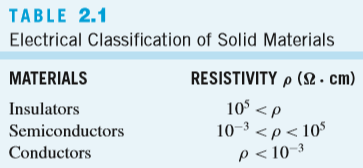
\includegraphics[width=0.8\linewidth]{img/ECSM.png}
        \caption{Eletrical Classification of Solid Materials} 
    \end{minipage}
    \begin{minipage}[htbp]{0.5\textwidth}
    \centering

    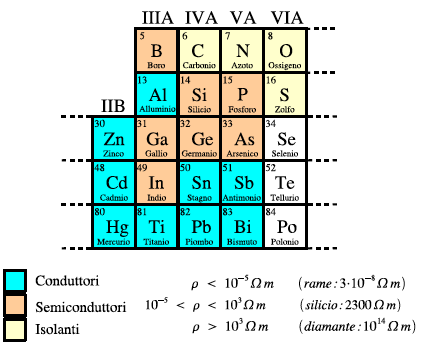
\includegraphics[width=0.8\linewidth]{img/TavolaPeriodica.png}    

    
    \end{minipage}
\end{figure}



% \begin{figure}[htbp]
%     \centering
%     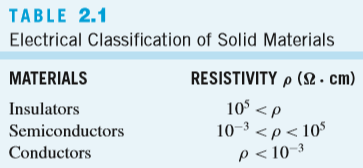
\includegraphics[width=0.4\linewidth]{img/ECSM.png}
%     \caption{Eletrical Classification of Solid Materials}    
% \end{figure}

% \begin{figure}[htbp]
%     \centering
%     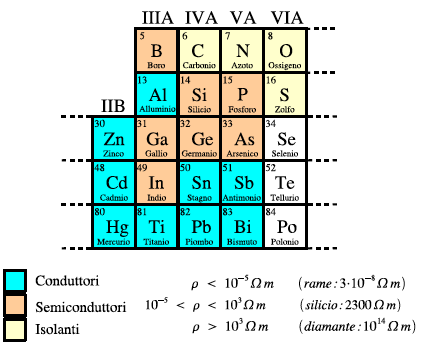
\includegraphics[width=0.55\linewidth]{img/TavolaPeriodica.png}    
% \end{figure}

\paragraph{Esempio:} Prendiamo un filo lungo 1 cm, area $10\mu m \cdot 10\mu m$. $L/A = 1/0.001\cdot0.001 = 10^6$

Prendendo come resistività $\rho = 10^5$ e poi $\rho = 10^{-3}$ ed utilizzando la relazione $\rho = R \frac{A}{L}$, otteniamo dei valori di resistenza di diversi ordini di grandezza differenti: $R = 100\,G\Omega \hspace{0.5cm} 1K\Omega$.

\newpage
\subsection{Struttura cristallina del silicio}
\begin{figure}[htbp]
    \centering
    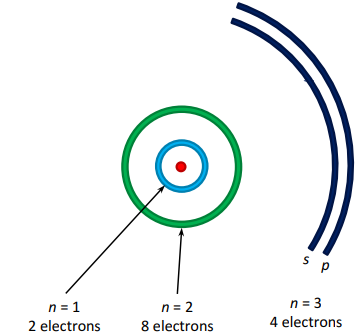
\includegraphics[width=0.35\linewidth]{img/silicio.png}
    \caption{Atomo di silicio}
    
\end{figure}

Alla temperatura dello zero assoluto, $0^{\circ}\,K = -273.15^{\circ}\,C$, tutti gli elettroni sono fissi in un legame covalente e dunque il materiale risulta isolante. Questo dovuto al fatto che nessuna carica, elettrone, si può muovere.

A temperature più alte, fornendo quindi dell'energia, alcuni legami si rompono e l'elettrone, sull'orbitale più esterno, è libero per la conduzione.


\begin{figure}[htbp]
    \centering
    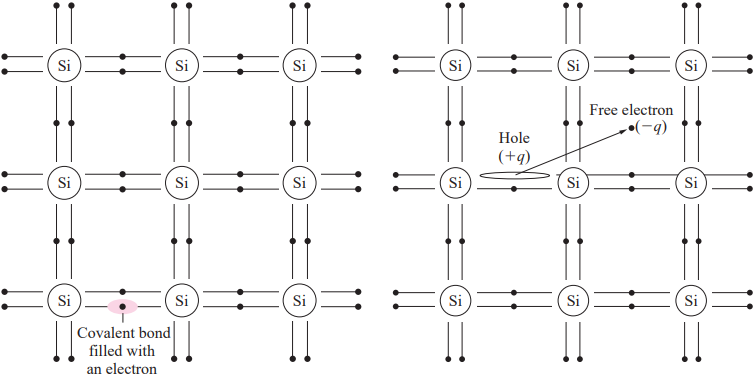
\includegraphics[width=0.8\linewidth]{img/legameSilicio.png}
    \caption{Struttura cristallina Silicio}    
\end{figure}


A questo punto si vede anche in figura che un elettrone che si stacca da un legame covalente lascia dietro di se un buco chiamato \textbf{hole} o \textbf{lacuna} che dovrà essere riempito.

\subsection{Densità di elettroni liberi}
Il numero di elettroni liberi in dipende da due fattori:
\begin{itemize}
    \item Temperatura;
    \item Materiale;
\end{itemize}


Utilizzando la seguente formula si possono trovare la densità di cariche:

\begin{equation}
    n_i^2 = BT^3\exp -\frac{E_G}{kT} 
\end{equation}

dove:
\newpage
\begin{itemize}
    \item $n_i = $ concentrazione di elettroni per $cm^3$
    \item $E_G = $ semiconductor bandgapenergy [$eV$] (elettronvolt, energia minima per rompere un legame)
    \item $k = $ costante di Boltzmann equivalente a $8.62 10^{-5}\,\,\,[eV/K]$
    \item $T = $ temperatura, [$K$]
    \item $B =$ parametro del materiale, $1.08 10^{31}\,\,\,[K^{-3}cm^{-6}] $ per il Si
\end{itemize}

\begin{figure}[htbp]
    \centering
    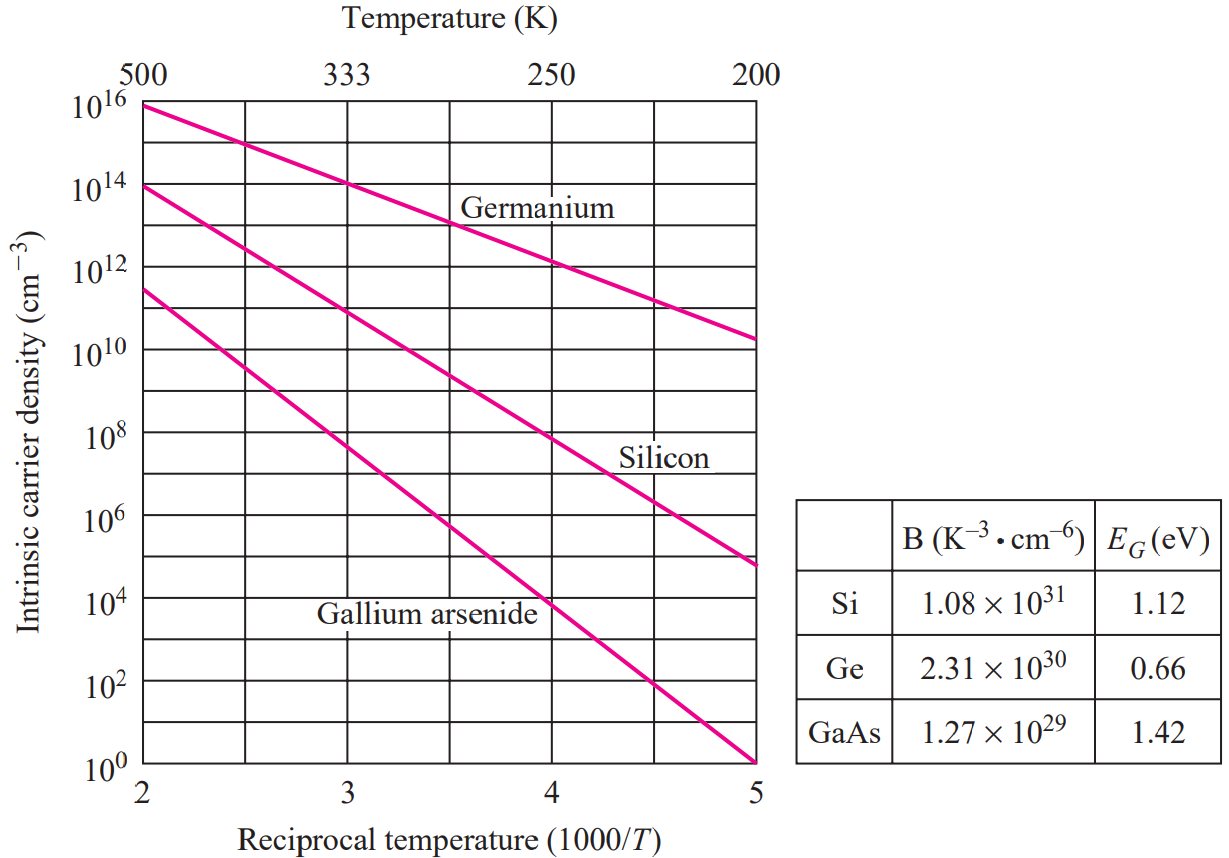
\includegraphics[width=0.75\linewidth]{img/bandGap.png} 
\end{figure}

\paragraph{Calcoliamo le cariche nel silicio:}

Sappiamo che la densità del silicio è: $5 10^{22} /cm^{3}$, applicando la formula a temperatura ambiente otteniamo:

\begin{equation*}
    n_i = 6.73 10^9 \approx 10^{10} /cm^3
\end{equation*}

\paragraph{Lacune: }
Un elettrone libero lascia dietro di se un buco, il quale dovrà essere riempito. Un elettrone da un altro legame può riempire il buco, che si sposta dalla parte opposta all'elettrone.

La lacuna la possiamo considerare come una carica \textbf{positiva}.
\paragraph{}
All'equilibrio, la densità di elettroni liberi e di lacune è identica.

\begin{equation*}
    n = n_1 = p \quad pn = n_i^2
\end{equation*}

dove 
\begin{itemize}
    \item n = concentrazione di elettroni liberi al $cm^3$;
    \item $n_1$ = numero di elettroni al $cm^3$, densità di e al$cm^3$;
    \item p = concentrazione di lacune libere al $cm^3$;
\end{itemize}

\begin{figure}[htbp]
    \centering
    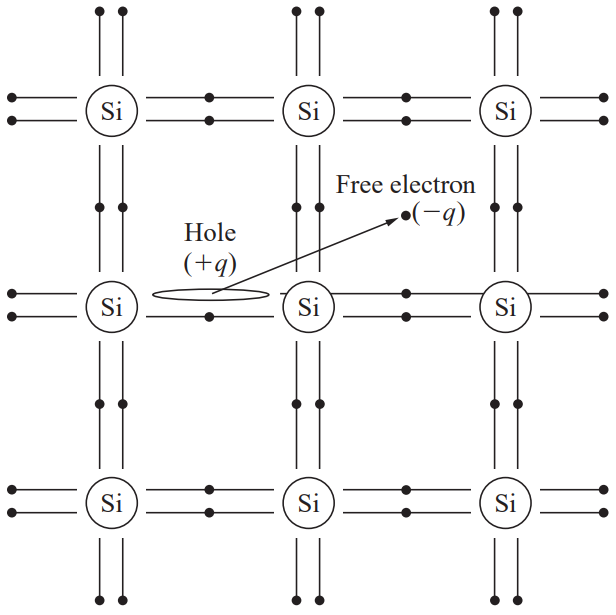
\includegraphics[width=0.4\linewidth]{img/hole.png}
    \caption{Spostamento di lacuna}    
\end{figure}

\newpage
\section{Corrente di drift}
Una elettrone libero, che rappresenta dunque una carica, può generare una corrente elettrica.

La corrente rappresenta la quantità \textbf{netta} di cariche per unità di tempo che attraversano la selezione del materiale. Il valore della corrente dipende dalla \textbf{velocità}. All'equilibrio termico, le cariche si muovono caoticamente e casualmente in tutte le direzioni, cambiando direzione ad ogni urto con un atomo del cristallo.

Questo fa si che:
\begin{itemize}
    \item La velocità media sia \textbf{nulla};
    \item La corrente totale risulti essere \textbf{zero}
\end{itemize}

\begin{figure}[htbp]
    \centering
    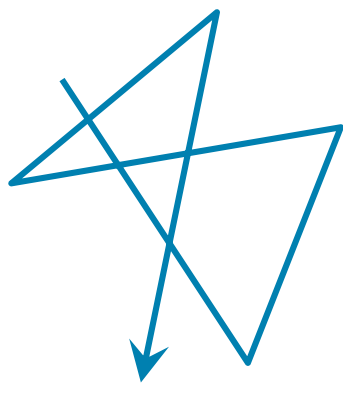
\includegraphics[width=0.14\linewidth]{img/moto-Casuale.png}    
\end{figure}


Applicando un \textbf{campo elettrico} E, le cariche tendono a muoversi nella sua direzione (drift).

\begin{itemize}
    \item Legge	di	Coulomb:\quad$\vec{F} = q\vec{E}$;
    \item Seconda	legge	di	Newton: \quad $\vec{F} = m\vec{a}$
    \item Quindi: $\vec{a} = \frac{q}{m}\vec{E}$
\end{itemize}

L'effetto della struttura dei materiali, essendoci gli atomi, fa si che le collisioni avvengano e modifichino la traiettoria dell'elettrone. Questo scontro fa perdere energia agli elettroni, effetto Jule, e l'effetto totale è quello di godere di un moto costante verso una direzione.

\begin{figure}[htbp]
    \centering
    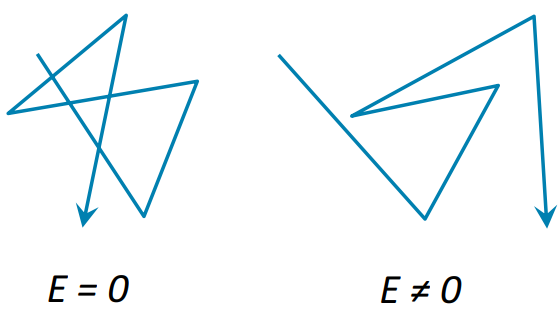
\includegraphics[width=0.33\linewidth]{img/campo_elettromagentico.png}  
\end{figure}

\newpage
La velocità risulta essere proporzionale al campo elettrico:

\begin{equation}
    v_n = -\mu_n\vec{E} \quad\quad v_p = \mu_p\vec{E}
\end{equation}

dove 
\begin{itemize}
    \item $v_n$ = Velocità elettroni
    \item $\mu_n$ = mobilità	degli	elettroni,	$1350\, cm^2/V\cdot s$	in	Si	intrinseco (puro).
    \item $v_p$ = Velocità lacune
    \item $\mu_p$ = mobilità	degli	elettroni,	$500\, cm^2/V \cdot s$	in	Si	intrinseco (puro).
\end{itemize}

Le	\textbf{lacune}	hanno	\textbf{minore	mobilità}	perché	costrette	a	muoversi	
nella	struttura,	mentre	gli	elettroni	godono di maggiore libertà.

\subsection{Velocità	di	saturazione}
Come visto prima, la velocità delle cariche risulta essere proporzionale, in media, al campo elettrico. Questo è vero fino ad un certo valore perché anche le cariche non possono superare la velocità	della luce, $300\,000\,\,\,[Km/s]$.

\paragraph{}
Dunque esiste un limite di saturazione il quale limita la risposta in frequenza e dunque anche la velocità di una porta logica (clock limitato).

\begin{figure}[htbp]
    \centering
    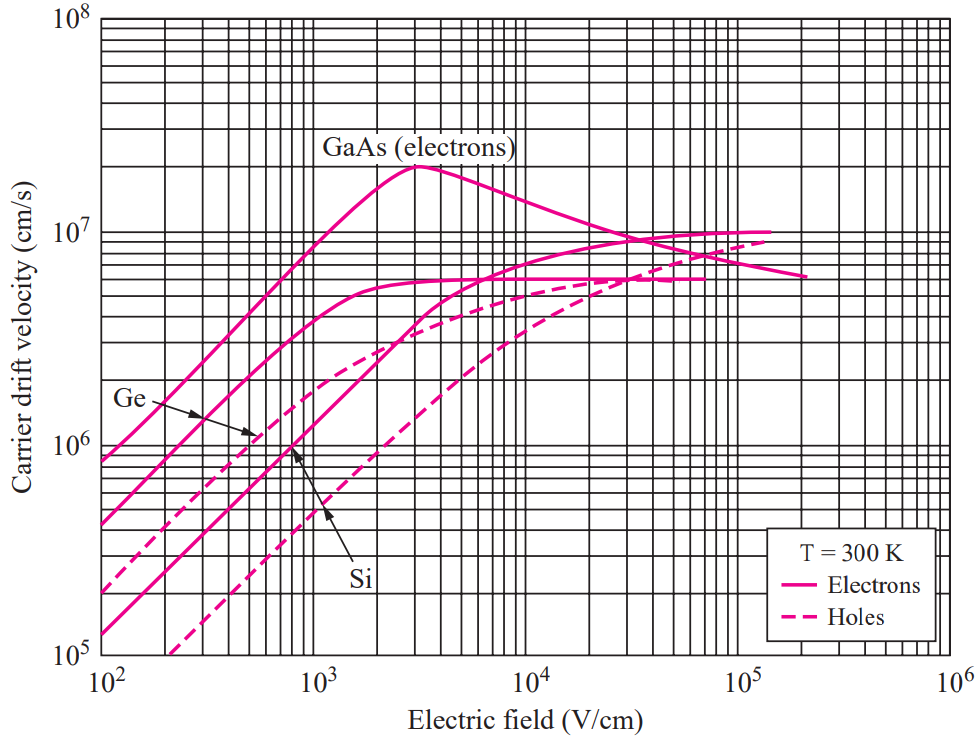
\includegraphics[width=0.75\linewidth]{img/saturazione.png}
    \caption{Velocità	di	saturazione}
\end{figure}

\newpage
\subsection{Calcolo della corrente di drift}
Valutiamo	la	carica	che	attraversa	una	superficie	nell'unità	di	tempo.


\begin{figure}[htbp]
    \centering
    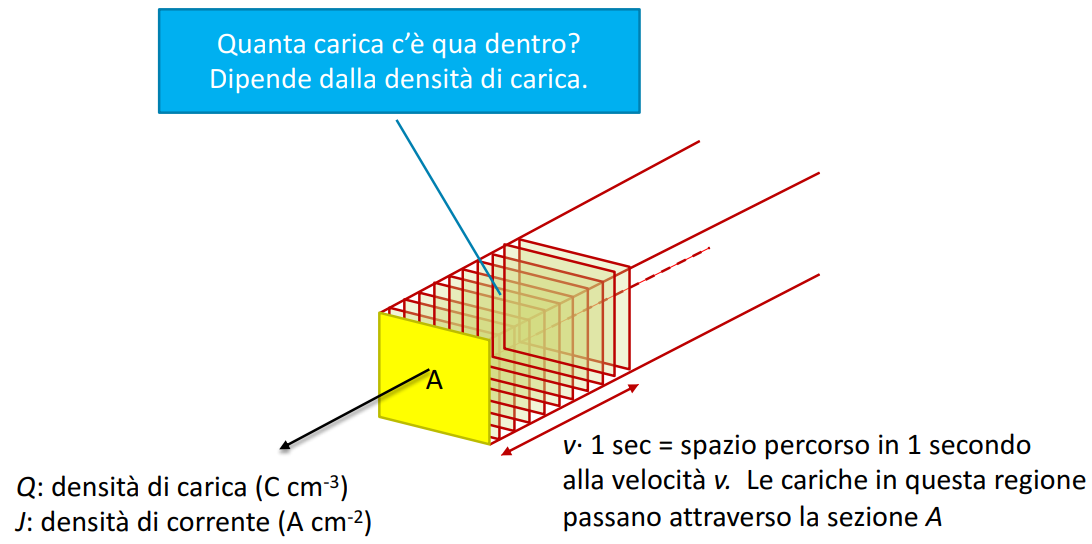
\includegraphics[width=0.9\linewidth]{img/carica_drift.png}
    \caption{Corrente di Drift}    
\end{figure}

Ricordiamo le seguenti formule:

\begin{equation*}
    I = JA = \sigma \frac{A}{L}\vec{E}L = GV \quad\quad q = 1.6\cdot10^{-19}
\end{equation*}
\begin{equation}
    j_n^{drift} = Q_nv_n = (-qn)(-\mu_n\vec{E}) = qn\mu_n\vec{E} \qquad[A/cm^2]
\end{equation}
\begin{equation}
    j_p^{drift} = Q_pv_p = (-qp)(-\mu_p\vec{E}) = qp\mu_n\vec{E} \qquad[A/cm^2]
\end{equation}
\begin{equation}
    j_T^{drift} = j_n^{drift} + j_p^{drift}Q_pv_p = q(n\mu_n + p\mu_p)\vec{E} = \sigma \vec{E}
\end{equation}

$\sigma: q(n\mu_n + p\mu_p)$ rappresenta la conduttività.

\paragraph{A temperatura ambiente}

\begin{itemize}
    \item[] $n = n_i = p = 10^{10}$
    \item[] $\sigma = (1.6*10^{-19})10^{10}(1350+500) = 2.96*10^{-6}$
\end{itemize}
\begin{equation*}
    j_T^{drift} = j_n^{drift} + j_p^{drift}Q_pv_p = q(n\mu_n + p\mu_p)\vec{E} = \sigma \vec{E}
\end{equation*}
\begin{equation*}
    \rho = \frac{1}{\sigma} = 3.38*10^{5}\, \omega cm
\end{equation*}

Dunque il silicio a temperatura ambiente rientra nella famiglia degli \textbf{isolanti}.

\paragraph{Conduttore in rame lungo 1m, di diametro 1mm e tensione di 1V}

\begin{itemize}
\centering
    \item[]  $R = \rho\frac{L}{A} = 1.68 10^{-8} \frac{1}{\pi 0.0005^2} = 0.0214 \,\omega$
    \item[]  $I = \frac{V}{R} = \frac{1}{0.0214} = 46.7\,A$
    \item [] $J = \frac{I}{A} = \frac{46.7}{\pi 0.0005^2 } = 59 10^6\,Am^{-2}$
    \item[]  $v = \frac{J}{nq} = \frac{59 10^6}{8.46 10^{28} 1.6 10^{-19}} = 0.0044 ms^{-1} = 4.4\,mms^{-1}$ 
\end{itemize}

Questa risulta essere la velocità netta di drift, gli elettroni si muovo a	velocità molto	più elevata,	ma	caoticamente.
Dunque gli elettroni impiegano delle ore per fare quale metro in un filo di rame, come è possibile dunque che la luce di una lampadina di accenda subito? 
\paragraph{}
Questo è dovuto alla \textbf{reazione a  catena} che da al via al tutto, e in generale è il \textbf{campo elettromagnetico} che si sposta rapidamente e che fa muovere gli elettroni.

\section{Impurità}
L'aggiunta	di	impurità	ci	permette	di controllare	la	resistività. 

\subsection{Atomi	pentavalenti }
Contribuiscono con un	elettrone	in	più, alcuni di questi atomi sono nella colonna V della tavola periodica:



\begin{itemize}
    \centering
    \item[] Fosforo, Arsenico, Antimonio
\end{itemize}




Questi atomi, superati i $0^{\circ}\,K$ , si ionizzano più velocemente ed essendo che hanno un elettrone in più, rispetto al Si, questo sarà libero di viaggiare libero nel reticolo cristallino. Essendo che P, As e Sb possono donare cariche, vengono chiamati \textbf{donatori}.

\subsection{Atomi	trivalenti }
Contribuiscono con un	\textbf{elettrone}	in	meno e dunque contribuiscono ad una \textbf{lacuna}, alcuni di questi atomi sono nella colonna III della tavola periodica:
\begin{itemize}
\centering
    \item[] Boro
\end{itemize}

Questi atomi, a differenza di quelli sopracitati, vengono chiamati \textbf{accettori} in quanto avendo sull'orbitale più esterni un elettrone in meno rispetto a Si, formano una lacuna la quale dovrà essere riempita da un elettrone del Si.
\paragraph{}
La conduzione è affidata prevalentemente a elettroni o lacune.

\paragraph{}
\begin{figure}[htbp]
    \centering
    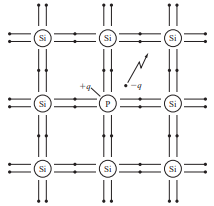
\includegraphics[width=0.35\linewidth]{img/energia_p.png}    
\end{figure}
Poca energia/calore è sufficiente per liberare le cariche, dunque queste impurità modificano la concentrazione di portatori:

\begin{itemize}
    \item $n = p$: Stiamo parlando del silicio senza impurità chiamato \textbf{intrinseco}
    \item $n \neq p$: Pariamo di silicio con aggiunta di impurità chiamato \textbf{estrinseco}
    \begin{itemize}
        \item[] $n > p$, il silicio è di \textbf{tipo n}, ovvero i portatori di maggioranza sono gli \textbf{elettroni}, donatori di ioni positivi. Questo silicio ha una migliore mobilità.
        \item[] $n < p$, il silicio è di \textbf{tipo p}, ovvero i portatori di maggioranza sono le \textbf{lacune}, donatori di ioni negativi. Questo silicio ha una peggiore mobilità.
    \end{itemize}
\end{itemize}
\newpage
\begin{figure}[htbp]
    \centering
    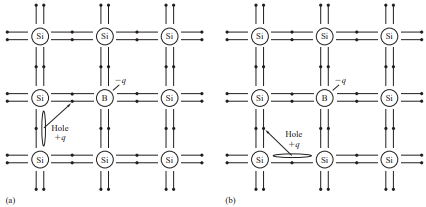
\includegraphics[width=0.75\linewidth]{img/boiro_energia.png}       
\end{figure}

\paragraph{}
Le concentrazioni di impurità sono normalmente dell'ordine di $10^{14}$ fino a $10^{21}$ atomi per $cm^3$, per confronto, la	concentrazione	intrinseca	di	portatori	è	dell'ordine	di	$10^{10}$ cariche	per	$cm^3$.
\paragraph{}
La	concentrazione	dei	portatori	\textbf{maggioritari} è	quindi	praticamente	uguale	alla	concentrazione	di	impurità	ed	è	
praticamente	costante. Sono le \textbf{impurità} che portano il più alto contenuto di elettroni liberi, l'equilibrio termico ne porta molte meno. Infatti aggiungere $10^{14}$ impurità significa aggiungere la stessa quantità di cariche o lacune.

\subsection{Conduzione}
Occorre	calcolare	la	concentrazione	di	portatori. La	carica	totale	del	conduttore	deve	essere	globalmente	nulla.
\begin{itemize}
    \item $N_D$ =	concentrazione	donatori	(ioni	positivi)
    \item $N_A$ =	concentrazione	accettori	(ioni	negativi)
\end{itemize}
\begin{equation*}
    q(N_D + p - N_A - n) = 0
\end{equation*}

Vale ancora la relazione (legge dell'azione di massa): $pn = n^2_i$
\paragraph{}
Quindi per i semiconduttori di tipo n: 
\begin{equation*}
    n^2 - (N_D - N_A)n - n_i^2\qquad n = \frac{(N_D - N_A) + \sqrt{(N_D - N_A)^2 + 4n_i^2}}{2}
\end{equation*}

In pratica se $(N_D - N_A) >> 2n_i$ allora:
\begin{equation*}
    n = N_D - N_A\qquad p = \frac{n_i^2}{n}
\end{equation*}

\subsubsection{Per il silicio di tipo p:}
\begin{equation*}
    p = N_A - N_D\qquad n = \frac{n_i^2}{p}
\end{equation*}

\paragraph{Pertanto:}
La	concentrazione	dei	portatori	\textbf{maggioritari}	è	praticamente	costante e	\textbf{indipendente	dalla	temperatura}.

La	concentrazione	dei	portatori	\textbf{minoritari} è	invece	proporzionale	a	$n_i^2$ e	fortemente \textbf{dipende		dalla	temperatura}

Per	esempio,	drogando	con	Boro	a	$10^{16}/cm^3$  e	con	Fosforo	a	$2\cdot10^{15}/cm^3$ a	temperatura	ambiente:

\begin{equation*}
    N_A = 10^{16} \qquad N_D = 2\cdot10^{15}
\end{equation*}
\begin{equation*}
   p = (N_A - N_D) = 8.00 \cdot 10^{15}
\end{equation*}
\begin{equation*}
   n = \frac{n_i^2}{p} = 1.25 \cdot 10^{4}
\end{equation*}

\paragraph{A 400 Kelvin (126,85°C):}
\begin{equation*}
   n_i^2 = 5.4 \cdot10^{24} \qquad p = (N_A - N_D) = 8.00\cdot10^{15} \qquad n = \frac{n_i^2}{p} = 6.75 \cdot 10^{8}
\end{equation*}


\subsection{Resistività in materiali estrinseci}
Il	drogaggio	riduce	la	mobilità	dei	portatori, infatti un silicio drogato con $N_D = 2\cdot10^{15}/cm^3$

\begin{equation*}
    n = 2\cdot10^{15}/cm^3 \qquad p = 10^{20}/2\cdot10\cdot10^{15} = 5\cdot10^{4}/cm^3
\end{equation*}

Questo silicio di tipo p ha una mobilità inferiore:
\begin{equation*}
    \mu_n = 1320\qquad\mu_p = 460
\end{equation*}

La conduttività e resistività sono:

\begin{equation*}
    \sigma = (1.6\cdot10^{-19})[(2\cdot10^{15})1320 + (5\cdot10^4)460] = 0.422
\end{equation*}

\begin{equation*}
    \rho = 1/\sigma = 2.37\,\,\,[\Omega cm]
\end{equation*}

Il silicio ora è un semiconduttore, da notare che una piccola frazione di impurità ($2\cdot10^{15} \text{ contro } 5\cdot10^{22}$) cambia la resistività di 5 ordini di grandezza, prima era: $3.38\cdot10^{5}$.

Dunque possiamo controllare la resistività del silicio.

\begin{figure}[htbp]
    \centering
    \includegraphics[width=0.65\linewidth]{img/resistività_SI.png}    
\end{figure}

\newpage
\section{Corrente di diffusione}
Se	il	drogaggio	non	è	uniforme	le	concentrazioni	dei	portatori	
variano	lungo	il	cristallo. Si	generano	quindi	correnti	di	diffusione	proporzionali	al	gradiente	di	
concentrazione.

\paragraph{}
I	portatori	vanno	da	regioni	a	maggiore	concentrazione	a	regioni	a minore	concentrazione, proprio come succede con lo scambio termico.
\begin{figure}[htbp]
    \centering
    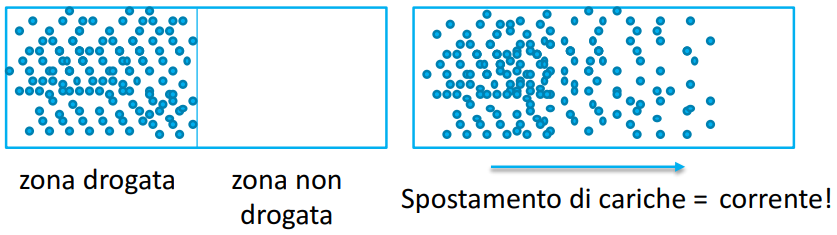
\includegraphics[width=0.7\linewidth]{img/corrente_diff.png}
\end{figure}

Si è notato che questa corrente di diffusione segue le seguenti ugualianze:

\begin{equation*}
    J_p^{diff} = (+q)D_p\biggl(-\frac{\partial p}{\partial x} = -qD_p\frac{\partial p}{\partial x}\biggl)
\end{equation*}
\begin{equation*}
    J_n^{diff} = (-q)D_n\biggl(-\frac{\partial n}{\partial x} = -qD_n\frac{\partial n}{\partial x}\biggl)
\end{equation*}
Dove $D_p \text{ e } D_n$ sono le diffusività	di	lacune	ed	elettroni	che	dipendono	dalla	
mobilità	e	temperatura	secondo	la	relazione	di	Einstein:

\begin{equation*}
    \frac{D_n}{\mu_n} = \frac{kT}{q} = \frac{D_p}{\mu_p} \qquad \text{ dove } V_t = kT/q = 0.0258V \text{ a } 300K
\end{equation*}

\section{Corrente totale}

Per ottenere la corrente totale, applicando un campo elettrico, dobbiamo sommare la corrente di drift e di diffusione:
\begin{equation}
    j_n^T = q\mu_nn\vec{E} + qD_n\frac{\partial n}{\partial x}
\end{equation}
\begin{equation}
    j_p^T = q\mu_pp\vec{E} + qD_p\frac{\partial p}{\partial x}
\end{equation}

Oppure applicando la relazione di Einstein: 
\begin{equation}
    j_n^T = q\mu_nn\biggl(\vec{E} + V_T\frac{1}{n}\frac{\partial n}{\partial x}\biggl)
\end{equation}
\begin{equation}
    j_p^T = q\mu_pp\biggl(\vec{E} - V_T\frac{1}{p}\frac{\partial p}{\partial x}\biggl)
    \label{eq_eine}
\end{equation}

Per completare il sistema dobbiamo considerare	la	dipendenza	del	campo	dalla	carica:

\begin{equation*}
    \nabla \cdot \varepsilon \vec{E} = Q
\end{equation*}

Dove $\varepsilon$ è la permittività e Q la	densità	di	carica	nello	spazio.

\newpage
\section{Take away}
Tramite	il	drogaggio	possiamo	controllare	la	
concentrazione	delle	cariche	nel	silicio, cariche	costituite	da	\textbf{elettroni}	e/o	\textbf{lacune}.
\paragraph{}
La corrente si può dividere in due componenti:
\begin{itemize}
    \item Corrente	di	\textbf{drift} dovuta	ad	un	campo	elettrico	applicato;
    \item Corrente	di	\textbf{diffusione} dovuta	a	gradienti	di	concentrazione.
\end{itemize}

I	dispositivi	elettronici	sono	realizzati	tramite	aree	di	tipo	
p	ed	n	collegate.

\section{Processo costruttivo}
I	circuiti	sono/erano	realizzati	secondo	un	processo	planare. Un	substrato	di	silicio	drogato	di	tipo	p	o	n	funge	da	supporto, altre aree	drogate	diversamente	di	tipo	p	o	n	vengono	create	sulla	superficie.

Queste	aree	sono	collegate	tra	loro	tramite	piste	in	alluminio,	
disposte	su	diversi	strati	separati	da	isolante.

\begin{figure}[htbp]
    \centering
    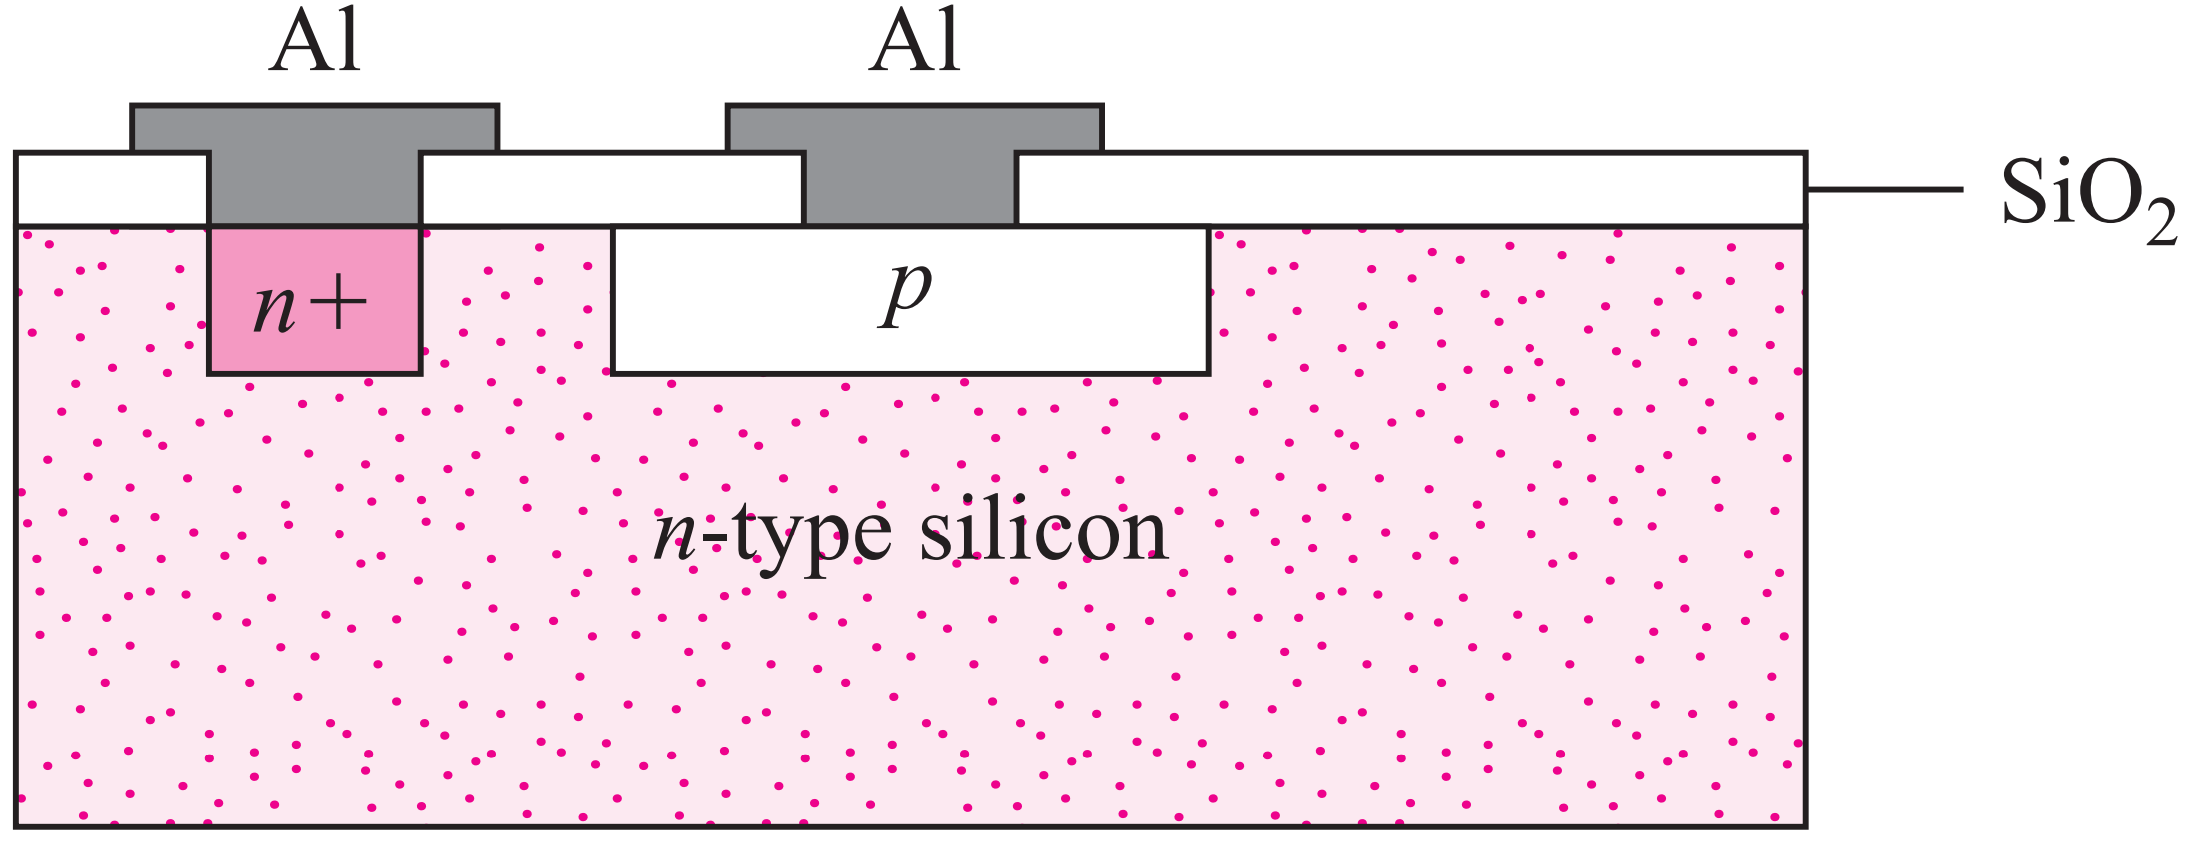
\includegraphics[width=0.45\linewidth]{img/transistor_costruzione.png}
    \caption{ Transistor vista frontale}    
\end{figure}

\chapter{Il Diodo}
\section{Come è fatto}

Il diodo è costruito	da	una	giunzione	di	silicio	di	tipo	p	e	n.
\begin{figure}[htbp]
    \centering
    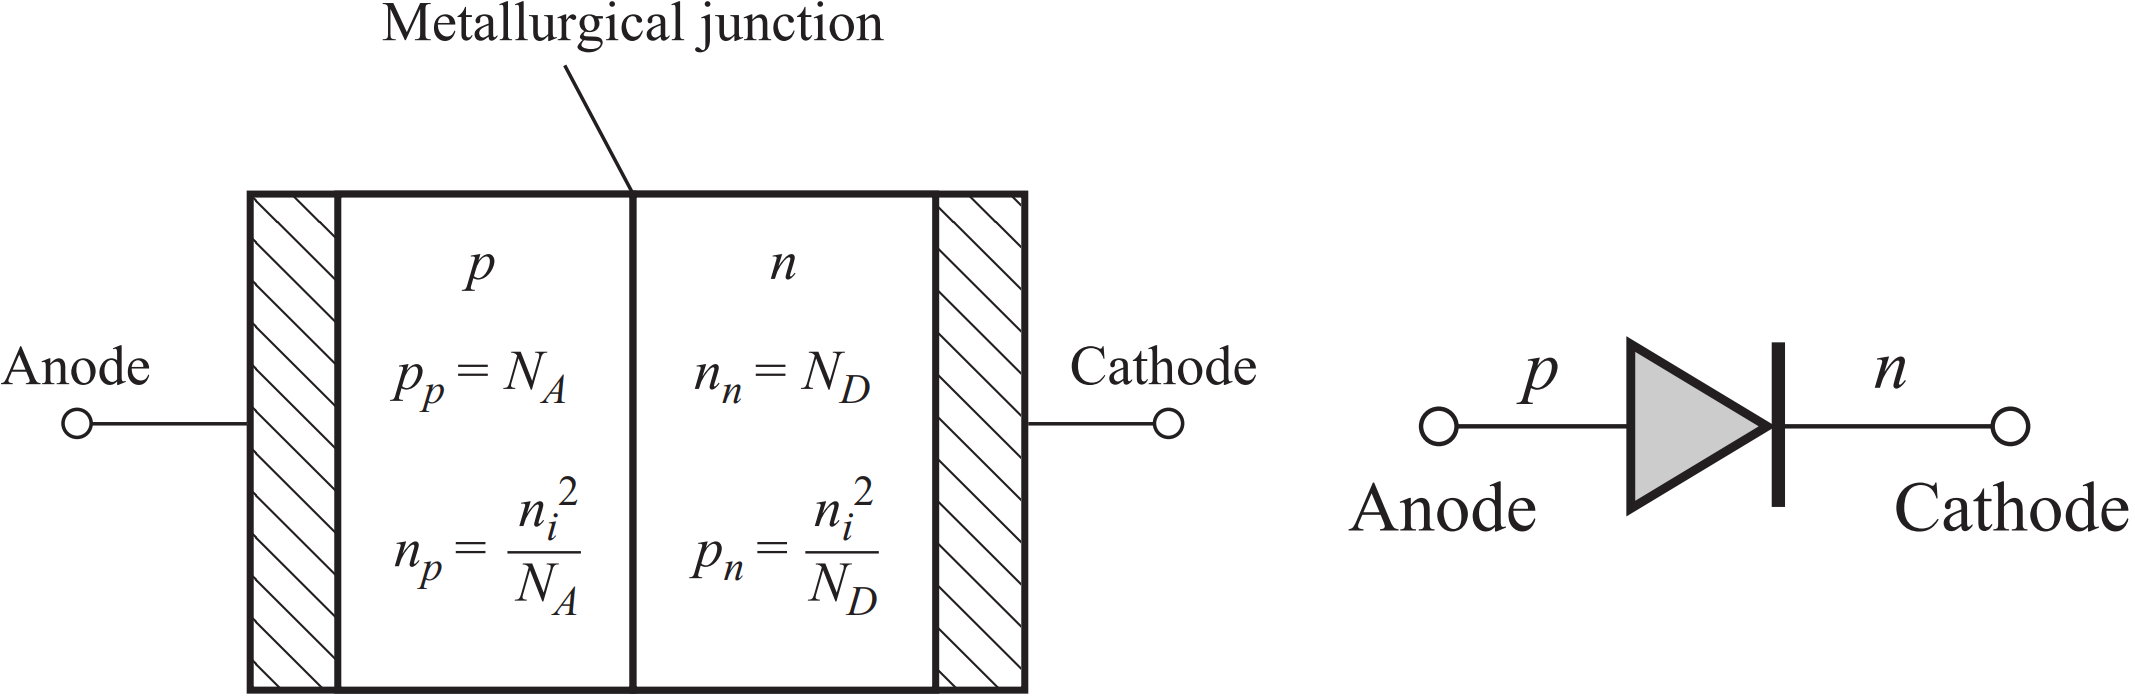
\includegraphics[width=0.65\linewidth]{img/diodo.png}
    \caption{Diodo}    
\end{figure}

Supponiamo 
\begin{itemize}
    \item $N_a = p_p= 10^{17}/cm^3\qquad N_D = n_n= 10^{16}/cm^3$
    \item $n_p = 10^{3}/cm^3\qquad p_n = 10^{4}/cm^3$
\end{itemize}

C’è	un	forte	gradiente	di	concentrazione	di	carica, infatti le	lacune	tendono	a	diffondere	dalla	zona	p alla zona n, mentre  gli	elettroni	tendono	a	diffondere	dalla	zona	n alla zona p.

\subsubsection{Carica	spaziale: } La	corrente	totale	deve	però	essere	nulla, infatti una corrente	di	drift deve	bilanciare	quella	di	diffusione. La corrente di drift è dovuta alla	creazione	di	una	regione	di	carica	spaziale,	
che	genera	un	campo	elettrico.



\begin{figure}[htbp]
    \centering
    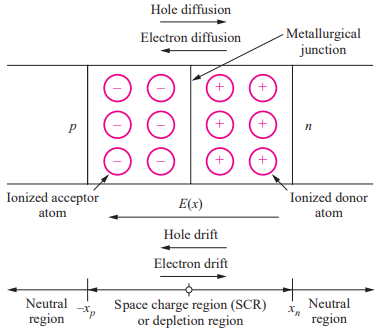
\includegraphics[width=0.45\linewidth]{img/corrente_spaziale.png}  
    
\end{figure}
\paragraph{}
Da dove viene il campo elettrico? A sinistra vi erano le lacune che si sono spostate nella parte n ed hanno lasciato degli atomi di Boro scoperti, questo fa si che si lasciano degli atomi ionizzati negativamente a sinistra. Gli elettroni che da destra sono andati a sinistra sono ioni positivi di fosforo.

Man mano che le cariche si diffondono, a ridosso della giunzione si forma una zona di ioni che sono cariche fisse e prendono in nome di \textbf{carica spaziale}, queste cariche fisse formano un dipolo con il positivo a destra e il negativo a sinistra formando così un campo elettrico dovuto a queste cariche.

Il CE fa insorgere una corrente di trascinamento che va in verso opposto a quelle della diffusione (il CE va dalle cariche positive a quelle negative, la corrente di diffusione il contrario).

\paragraph{}
Dunque all'inizio si forma la corrente di diffusione, e inizia a formarsi la carica spaziale a ridosso della giunzione e quest'ultima ostacola la diffusione ed ad un certo punto si arriva ad un equilibrio.

Questo equilibrio non significa che non c'è più movimento ma le cariche che diffondono e driftano si annullano a vicenda e dunque la corrente totale diventa nulla.

\begin{figure}[htbp]
    \centering
    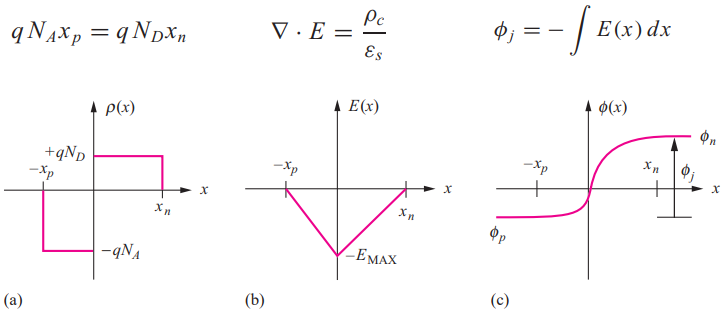
\includegraphics[width=0.9\linewidth]{img/carica_sapzoale_2.png}   
    
\end{figure}

Per capire quando questo processo va in equilibrio possiamo calcolare il campo elettrico. Possiamo calcolarlo perché la quantità di questi ioni, concentrazione, la sappiamo a priori dato che li abbiamo inseriti noi consapevolmente, sotto l'ipotesi che si siano tutti ionizzati.

\section{Calcolo del potenziale di built-in $\phi_j$}
Il potenziale di \textbf{built-in} è il fenomeno che si oppone alla diffusione delle cariche tra una zona e l'altra, viene chiamato di built-in perché è già all'interno dopo la giunzione dei due materiali con drogaggi diversi.
\paragraph{}
Sarà necessario \textbf{superare} questo potenziale per far scorrere una corrente all'interno del diodo facendolo lavorare come un corto circuito.

\paragraph{}
Utilizzando l'equazione \ref{eq_eine} e ponendola uguale a zero, dato che la corrente si deve bilanciare, avremo che:

\begin{equation*}
    E - V_T\frac{1}{p}\frac{\partial p}{\partial x} = 0 \qquad\longrightarrow\qquad E = -\frac{\partial V}{\partial x}
\end{equation*}
\begin{equation*}
    -\frac{\partial V}{\partial x} = V_T\frac{1}{p}\frac{\partial p}{\partial x}\qquad\longrightarrow\qquad dV = -V_T\frac{dp}{p}
\end{equation*}

integrando da ambo le parti otteniamo che:

\begin{equation}
    V_2 - V_1 = \phi_j = V_T\cdot \ln\biggl(\frac{N_AN_D}{n_i^2}\biggl)
\end{equation}

\newpage
dove:
\begin{itemize}
    \item $N_A \text{ e } N_D$ li conosciamo dato che abbiamo deciso noi le impurità
    \item $n_i$ dipende dalla temperatura
    \item $V_T$ è una costante
\end{itemize}
\begin{equation*}
    \phi_j = 0.026\ln(10^{17}10^{16}/10^{20}) = 0.026\ln(10^{13}) \approx 0.7V
\end{equation*}

Questo potenziale di built-in $\phi_j$ risulta essere circa $0.75V$ per il silicio e $0.3V$ per il germanio, tensione che contrasta la diffusione delle cariche dei portatori.

Questo significa che una lacuna a sinistra deve avere abbastanza energia per superare la barriera di potenziale.

\section{Potenziale esterno}

Applicando	un	potenziale	esterno	si	altera	l'equilibrio.

\begin{itemize}
    \item Un	\textbf{potenziale	positivo}	riduce	la	barriera,	e	una	corrente	può	scorrere	nel	diodo
    \item Un	\textbf{potenziale	negativo}	incrementa	la	barriera.	La	corrente	scorre,	ma	è	molto	piccola	perché	fatta	solo	dai	portatori	minoritari
\end{itemize}

Per la legge della sovrapposizione degli effetti il potenziale esterno si somma a quello interno.

\begin{figure}[htbp]
    \centering
    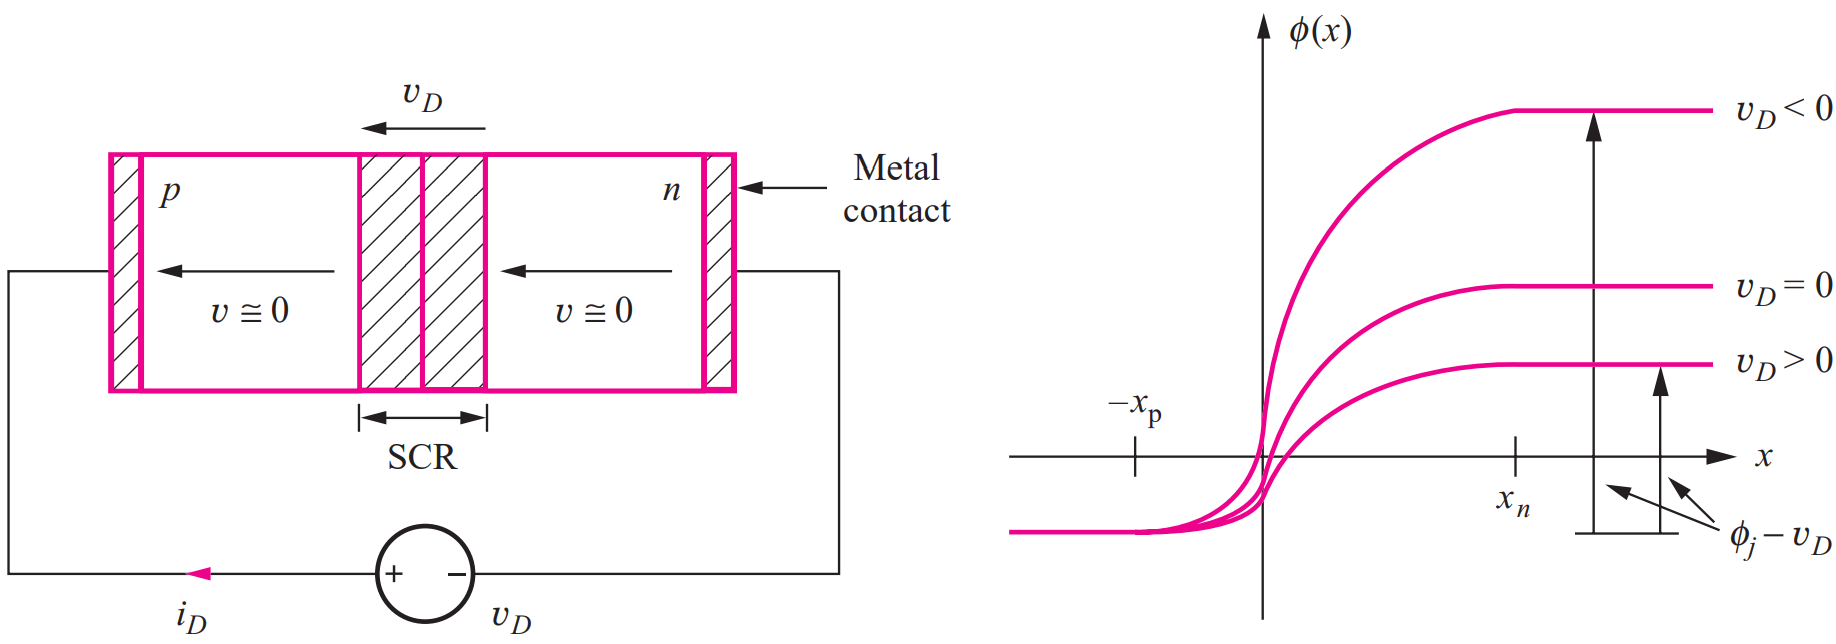
\includegraphics[width=0.9\linewidth]{img/pote_est.png}
    
    
\end{figure}

La barriera si può molto facilmente abbassare o azzerare, basta applicare una differenza di potenziale tra anodo e catodo di $0.7V$ e a questo punto tutte le cariche possono spostarsi liberamente.

\subsection{Potenziale	positivo}
L'equilibrio	è	perturbato,	la	regione	di	carica	spaziale	si	restringe, inoltre passerà molta corrente in quanto la differenza di densità di carica è di diversi ordini di grandezza superiore.

La	corrente	di	drift non	è	in	grado	di	bilanciare	quella	di	diffusione dunque:
\begin{itemize}
    \item le lacune si	diffondono	dalla	zona	p	alla	zona	n;
    \item gli elettroni si	diffondono	dalla	zona	n	alla	zona	p;
    \item le correnti fluiscono nello stesso verso.
\end{itemize}

\newpage
\subsection{Potenziale	negativo}
In questo caso mettiamo una batteria in polarità inversa: il $+$ sul catodo e il $-$ sull'anodo. Così facendo non solo le cariche sono contrastate dalla barriera di spostamento ma vi è anche la barriere aggiuntiva della batteria collegata e dunque le cariche non diffondono per niente e non passa corrente.

\paragraph{}
La	barriera	di	potenziale	si	amplia, la	regione	di	carica	spaziale	si	allarga. La	corrente	di	diffusione	viene	ostacolata,	mentre	i	portatori	minoritari	possono	scivolare	per	la	barriera:

\begin{itemize}
    \item le lacune si	diffondono	dalla	zona	n	alla	zona	p;
    \item gli elettroni si	diffondono	dalla	zona	p	alla	zona	n.
\end{itemize}

Scorre	quindi	una	debole	corrente,	dovuta	ai	portatori minoritari	generati	termicamente, in	prima	approssimazione	indipendente	dal	potenziale, talmente piccola che può essere considerata nulla.

\paragraph{}
Il diodo a differenza di un resistore permette di dare un solo verso alla corrente, \textbf{raddrizzarla}: infatti si para di \textbf{polarizzazione}.

\begin{itemize}
    \item \textbf{Polarizzazione diretta}: tensione esterna applicata in modo da ridurre la barriera energetica permettendo il flusso di corrente;
    \item \textbf{Polarizzazione inversa}: tensione esterna applicata in modo da aumentare la barriera energetica impedendo il flusso di corrente.
\end{itemize}


\begin{figure}[htbp]
    \centering
    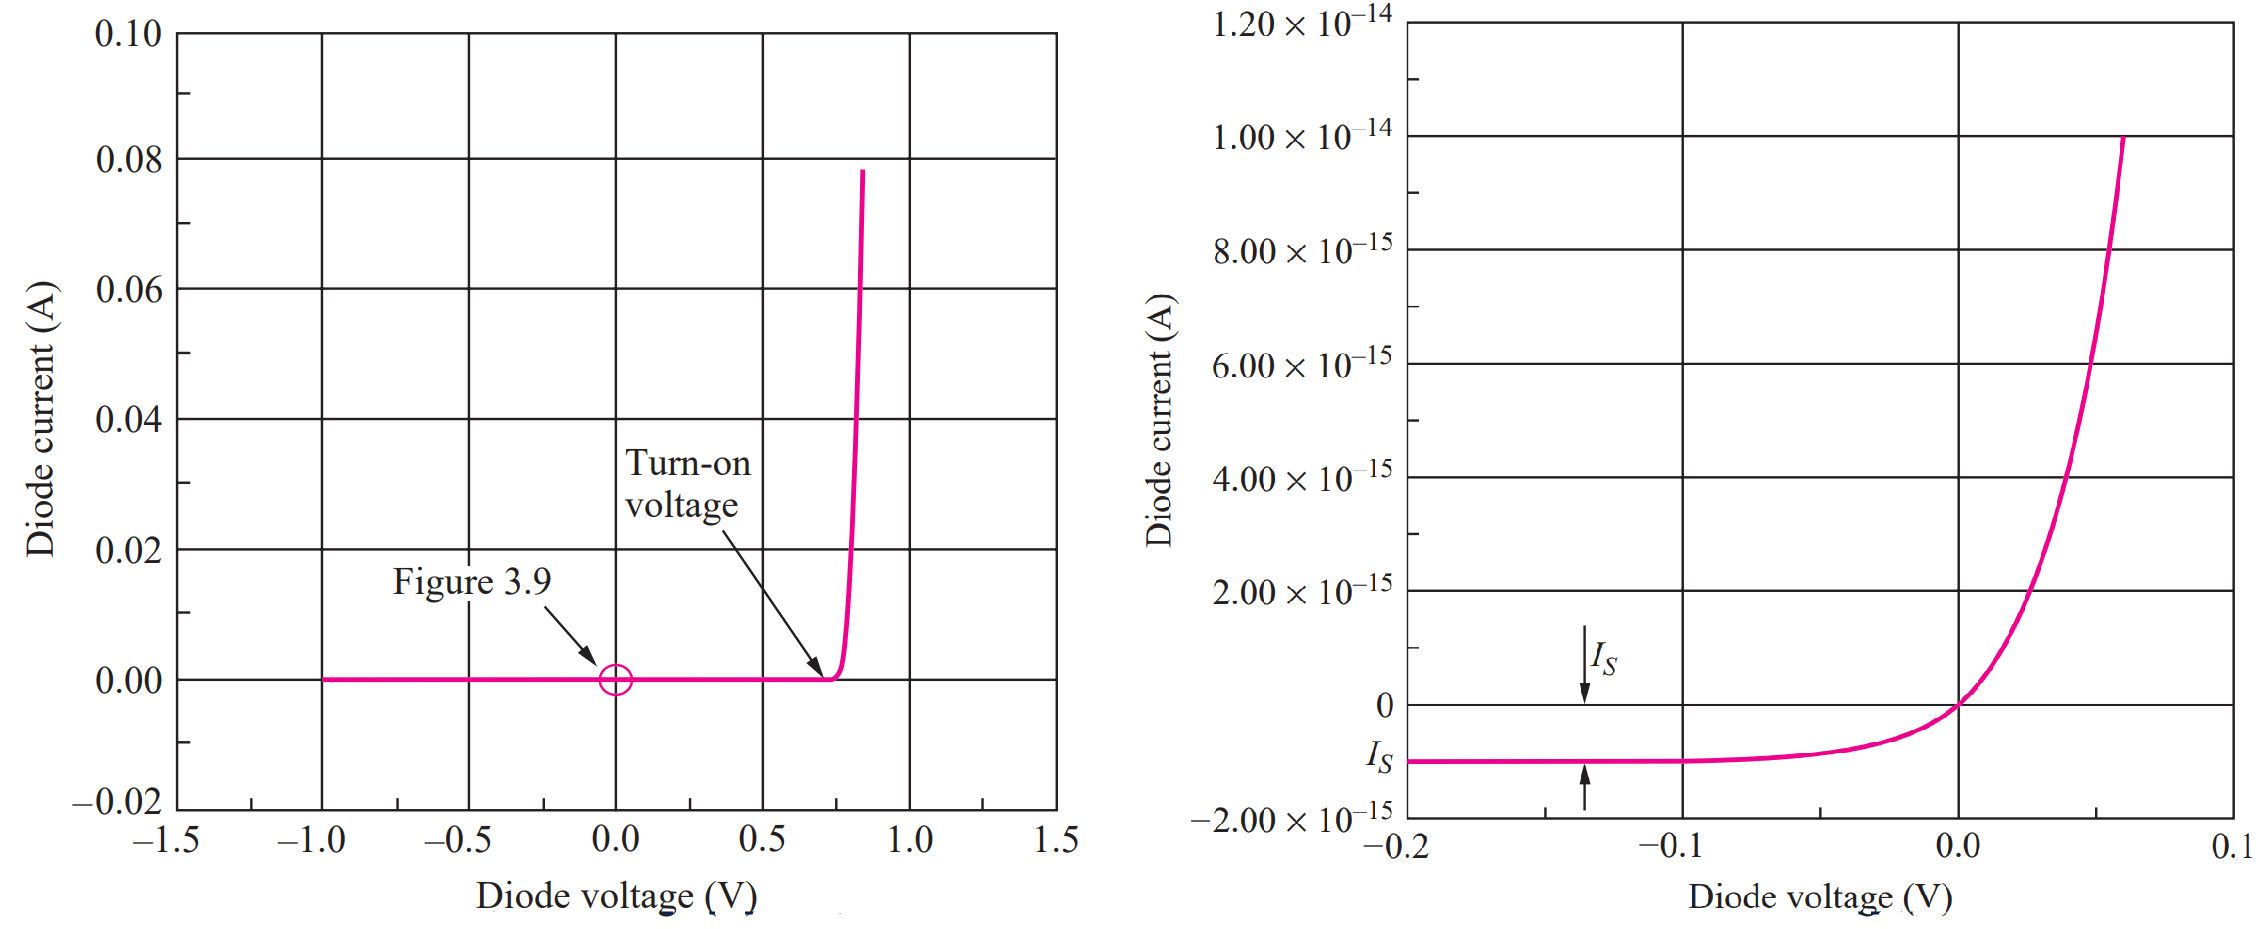
\includegraphics[width=0.97\linewidth]{img/potenziale_diodoi.png}
    \caption{Grafico andamento tensione-corrente}
    
\end{figure}

\newpage
\section{Modello matematico del Diodo}

\begin{equation}
    I_D = I_S\biggl[\exp{\biggl(\frac{qv_D}{nkT}\biggl)-1}\biggl] = I_S\biggl[\exp{\biggl(\frac{v_D}{nV_T}\biggl)-1}\biggl]
\end{equation}

Dove

\begin{itemize}
    \item $I_S$ =	corrente	inversa	di	saturazione
    \item $v_D$ =	tensione	applicata	ai	capi	del	diodo
    \item q = carica elettrone $1.6\cdot10^{-19} \text{ [C]}$
    \item k = costante	di	Boltzmann $1.38\cdot10^{-23} \text{ [J/K]}$
    \item n	=	fattore	di	non	idealità	(tipicamente	1 per Si)
    \item $V_T = kT/q$ = tensione termica (0.025V, Si, temp. amb)
\end{itemize}


\section{Modello di diodo ideale per grandi tensioni}
Quando si lavora con tensioni molto maggiori della tensione minima per far oltrepassare la barriera alle cariche (0.7V) allora possiamo applicare una prima approssimazione generale del diodo:
\begin{figure}[htbp]
    \centering
    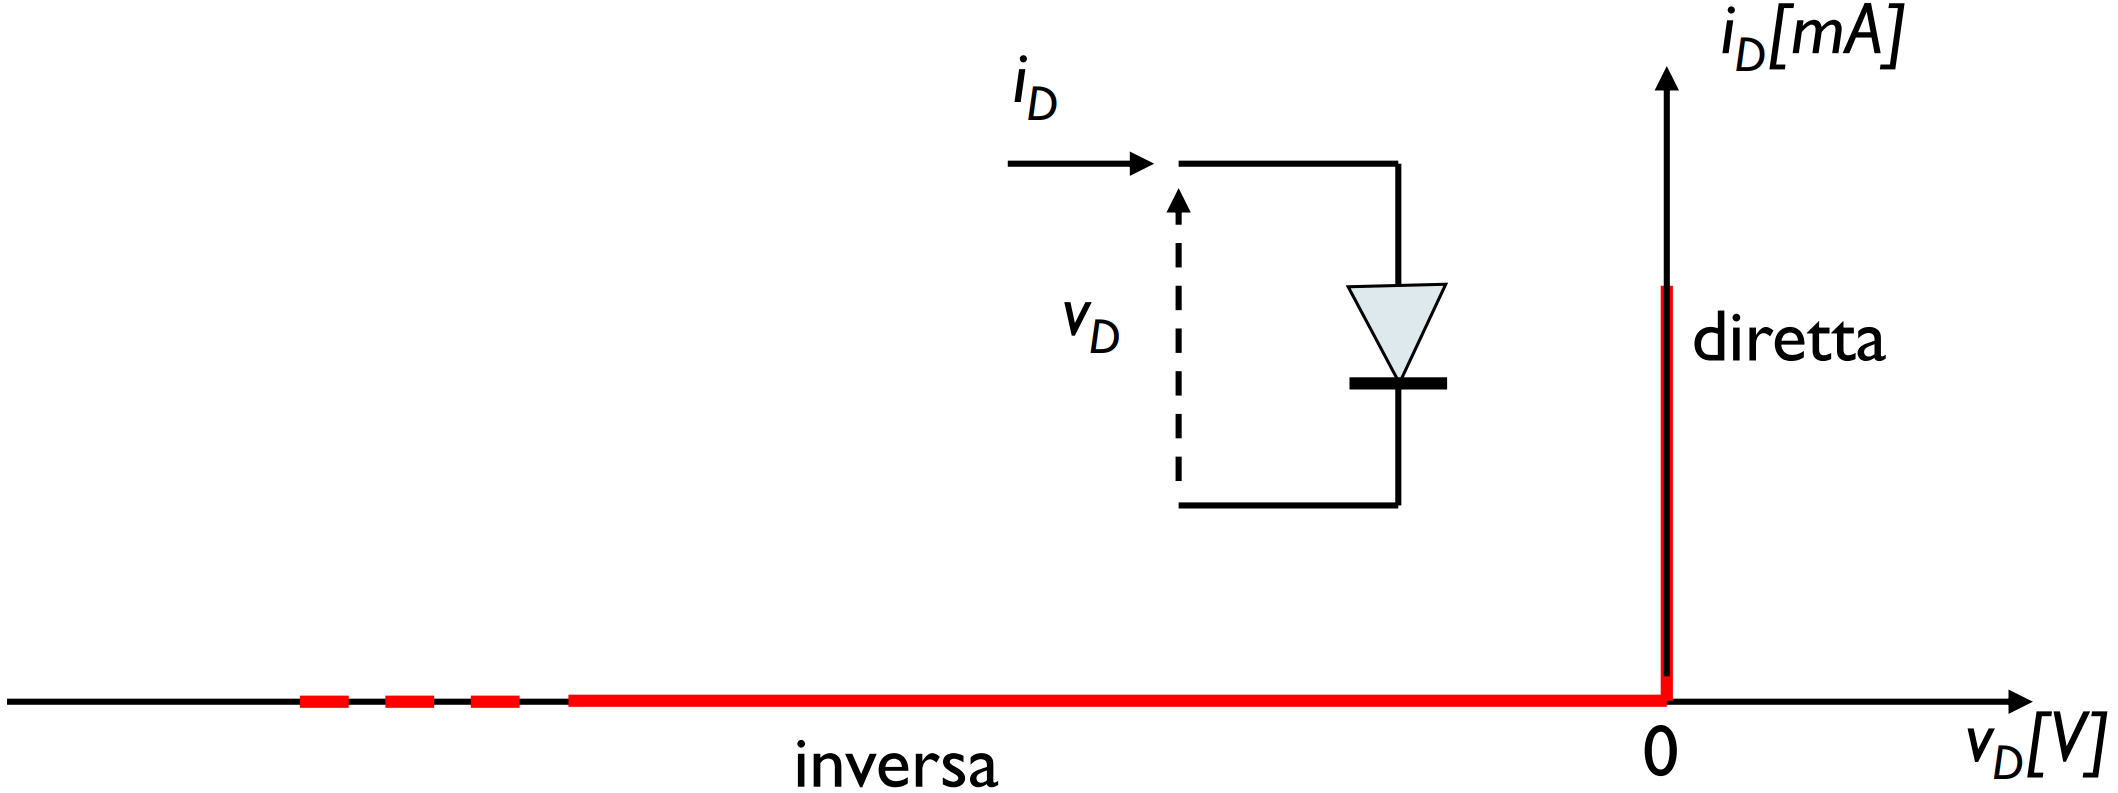
\includegraphics[width=0.65\linewidth]{img/diodo_Ideale.png}
    \caption{Diodo ideale}    
\end{figure}

\paragraph{}
Questa grossolana approssimazione è applicabile se il nostro circuito è sottoposto a decine di volt.
\begin{figure}[htbp]
    \centering
    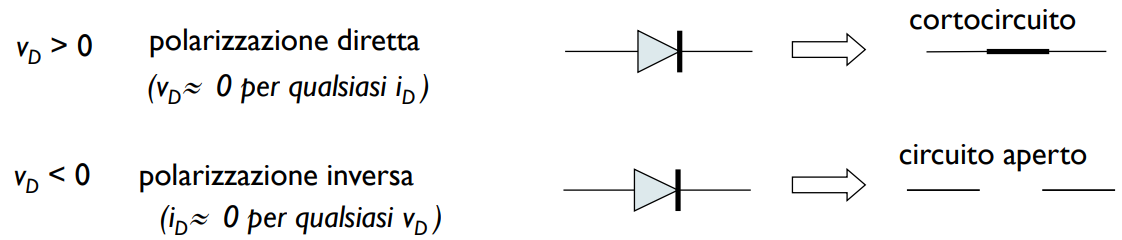
\includegraphics[width=0.77\linewidth]{img/approx_diodo.png}
    \caption{Comportamento in una rete}    
\end{figure}


\section{Diodo nei circuiti}

I diodi sono dei componenti molto utilizzati soprattutto negli alimentatori di apparecchiature elettroniche in quanto esse, funzionando in regime di corrente continua, hanno bisogno di rendere positiva la sinusoide di rete per poter poi estrarre, grazie ad un condensatore, la componente continua.
\paragraph{}
Vediamo alcuni esempi di circuiti.
\newpage
\subsection{Rettificatore a semi onda}
Il diodo è molto utilizzato per raddrizzare la sinusoide di rete.

\begin{figure}[htbp]
    \centering
    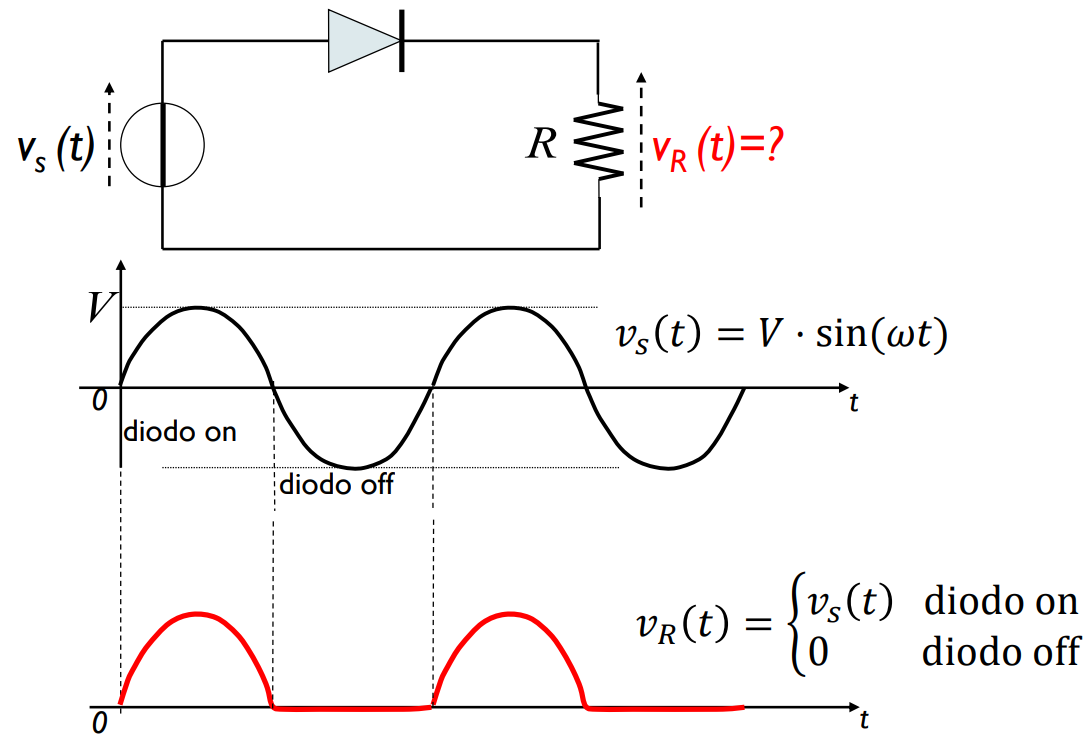
\includegraphics[width=0.7\linewidth]{img/rettificatore.png}
    \caption{Rettificatore a semi onda}    
\end{figure}

\paragraph{}
\subsection{Rettificatore ad onda intera, il ponte di diodi}
Ovviamente possiamo raddrizzare tutta la sinusoide di rete in una sinusoide con soli semi onde positive, grazie al ponte di diodi:

\begin{figure}[htbp]
    \centering
    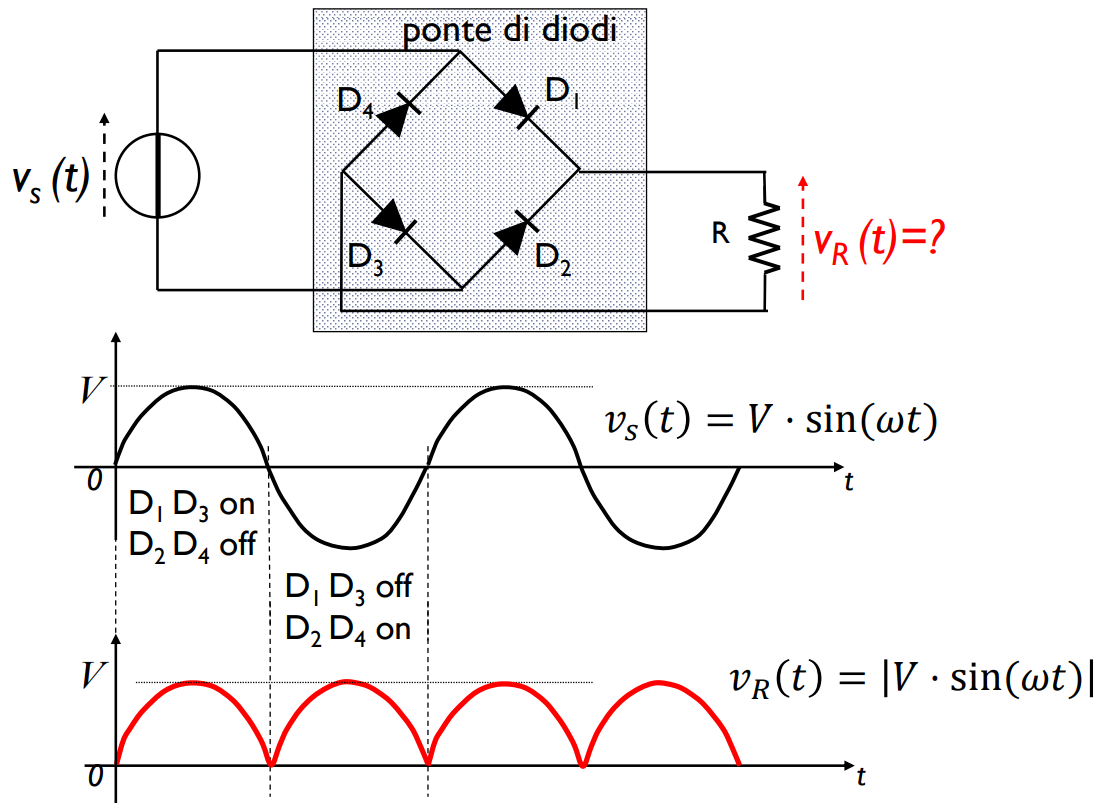
\includegraphics[width=0.65\linewidth]{img/ponte_diodi.png}
    \caption{Ponte di diodi}
    
\end{figure}

\paragraph{}
\subsection{Raddrizzatore AC/DC con filtro capacitivo}
Normalmente i dispositivi elettronici funzionano in corrente continua. La rete però fornisce una tensione sinusoidale a 50Hz.
Grazie al seguente circuito possiamo far tendere la nostra sinusoide di rete ad una tensione costante.

\begin{figure}[htbp]
    \centering
    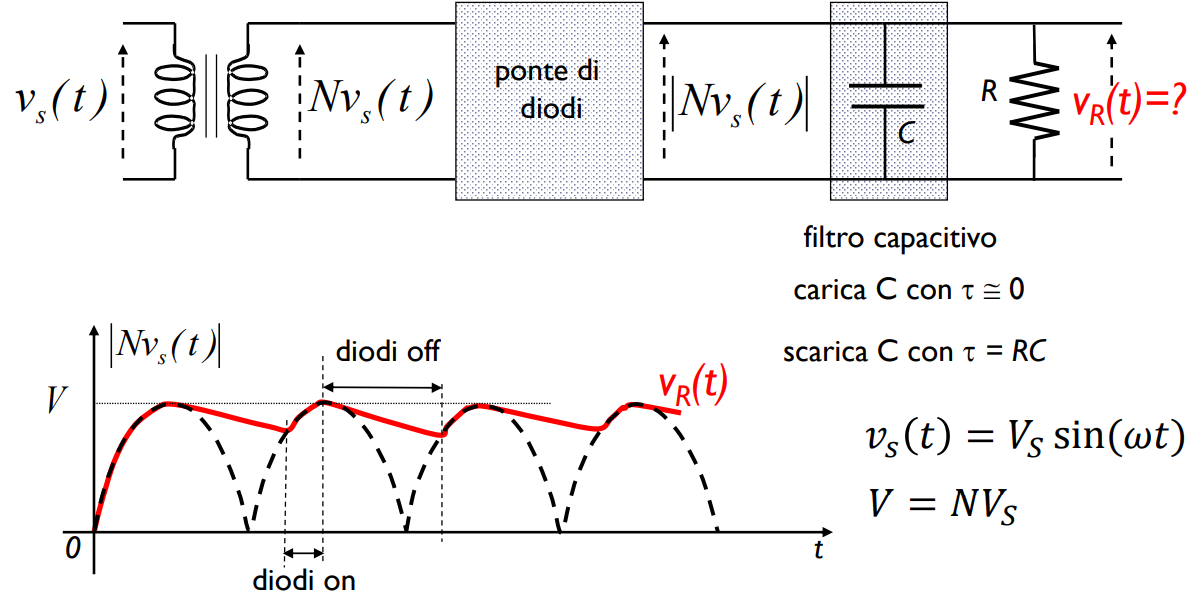
\includegraphics[width=0.75\linewidth]{img/raddrizzatore.png}
    \caption{Raddrizzatore AC/DC con filtro capacitivo}    
\end{figure}

La fluttuazione della tensione di uscita $V_R(t)$ può essere controllata
modificando la costante di tempo di scarica $\tau = RC$ ($>>T$)
\paragraph{}
Più il condensatore è grosso più riesce a mantenere costante la tensione durante la scarica, dunque perché non utilizzarne uno con molta capacità?
\paragraph{}
Ci sono alcuni motivi per evitare l'utilizzo di un condensatore grande:

\begin{itemize}
    \item \textbf{Corrente di carica elevata:} Un condensatore di grandi dimensioni richiede una corrente di carica elevata durante l'avvio del circuito. Questo può causare picchi di corrente eccessivi che possono danneggiare i diodi raddrizzatori e altri componenti del circuito.
    \item \textbf{Tempo di carica lungo:} Un condensatore di grandi dimensioni impiega più tempo per caricarsi. Questo può portare a un ritardo significativo nella tensione di uscita all'accensione del circuito.
    \item \textbf{Aumento del ripple:} Un condensatore di grandi dimensioni può aumentare il ripple della tensione di uscita. Il ripple è la componente alternata residua presente nella tensione continua dopo la raddrizzatura. Un ripple eccessivo può essere dannoso per i circuiti elettronici sensibili.
    \item \textbf{Dimensioni e costo:} Un condensatore di grandi dimensioni è più grande e costoso di un condensatore di dimensioni più ridotte.

    \item \textbf{Non adatto a carichi variabili:} Un condensatore di grandi dimensioni non è adatto a carichi variabili. Se il carico varia, la tensione di uscita varierà di conseguenza.
\end{itemize}

In generale, è consigliabile utilizzare un condensatore di dimensioni sufficienti per ridurre il ripple a un livello accettabile, ma non troppo grande da causare i problemi sopra menzionati. Il valore ottimale del condensatore dipende da diversi fattori, tra cui la frequenza della tensione di rete, il tipo di raddrizzatore, il valore del carico e il livello di ripple desiderato.


\newpage
\section{Modello di diodo ideale per piccole tensioni}

A differenza di prima ora stiamo prendendo in esame un circuito che lavora su basse tensioni (es. 5V). Per questo utilizzo non si può approssimare come prima in quanto la barriera di potenziale iniziale diventa molto rilevante e potrebbe creare problemi ai carichi che si attaccano al circuito.

\begin{figure}[htbp]
    \centering
    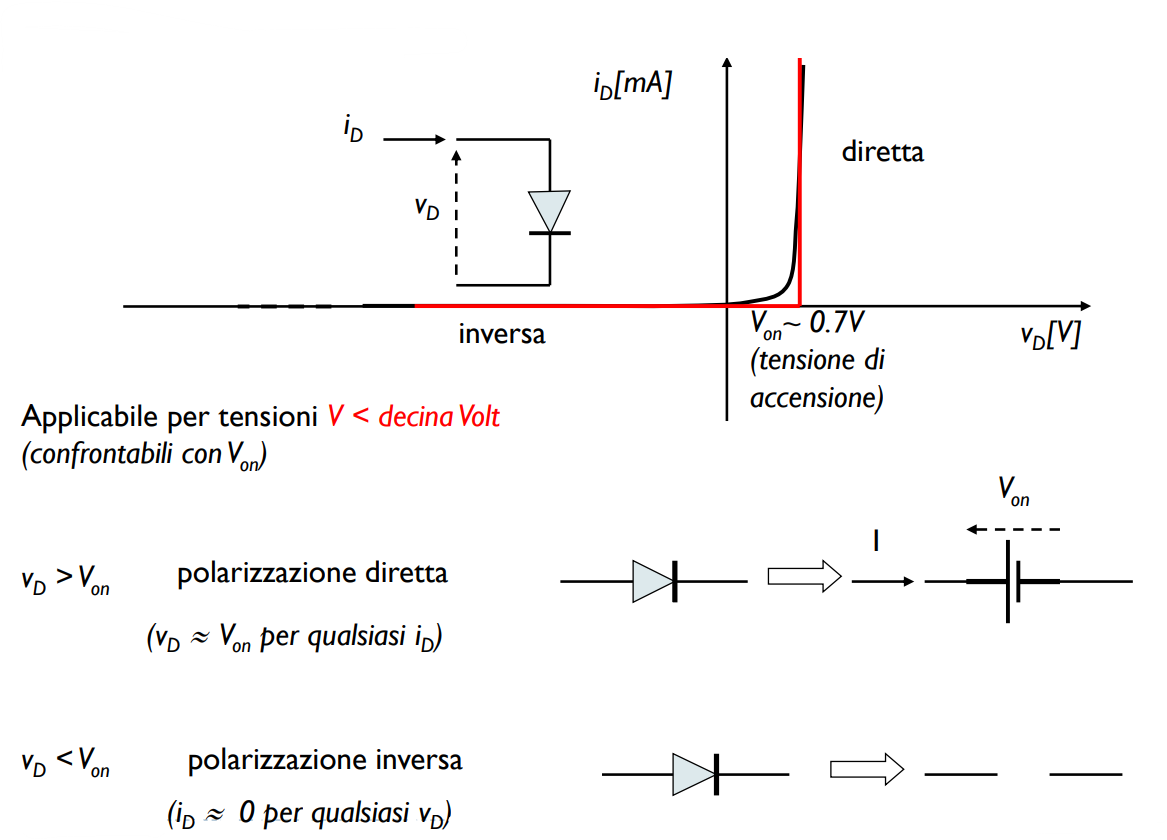
\includegraphics[width=0.8\linewidth]{img/piccole_tens.png}
    \caption{Modello di diodo per piccole tensioni}    
\end{figure}

\section{I circuiti logici realizzabili con i diodi}
I diodi possono essere utilizzati per costruire porte logiche quali ad esempio la AND e OR.
\paragraph{}

Di seguito verrà mostrata una loro possibile implementazione.
\newpage
\subsection{Circuito AND}

\begin{figure}[htbp]
    \centering
    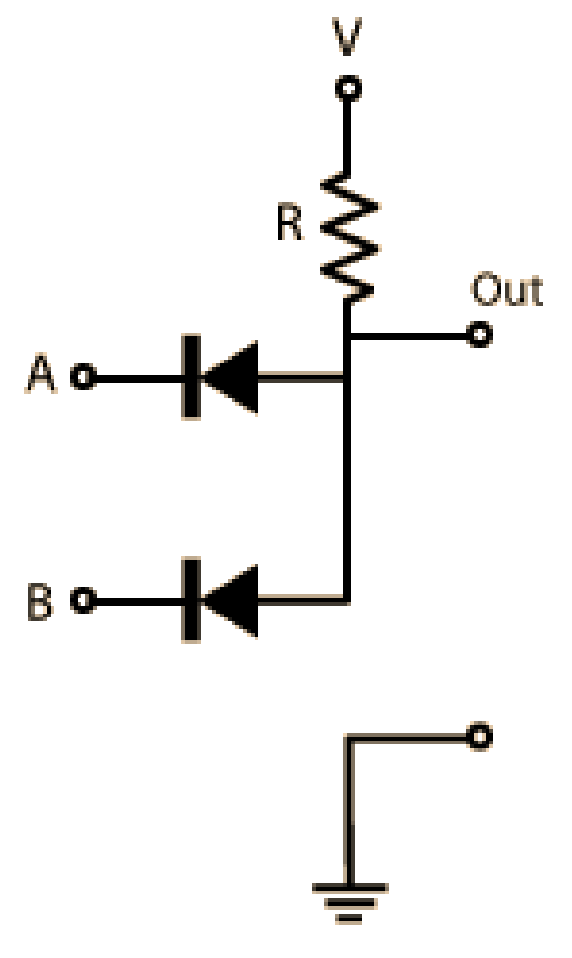
\includegraphics[width=0.17\linewidth]{img/and.png}
    \caption{Diode AND gate}
    
\end{figure}

Vediamo i tre casi:

\begin{itemize}
    \item $V_A = V_B = 5V$
    \begin{itemize}
        \item entrambi i diodi sono interdetti
        \item non scorre corrente 
        \item l'uscita va a 5V
    \end{itemize}
    \item $V_A = 0V,  V_B = 5V$
    \begin{itemize}
        \item Il diodo B conduce, il diodo A è interdetto
        \item l'uscita scende a $V_{on}$ (0 per grandi tensioni)
    \end{itemize}
    \item $V_A = V_B = 0V$
    \begin{itemize}
        \item entrambi i diodi conducono
        \item l'uscita scende a $V_{on}$ (0 per grandi tensioni)
    \end{itemize}
\end{itemize}

\subsection{Circuito OR}
\begin{figure}[htbp]
    \centering
    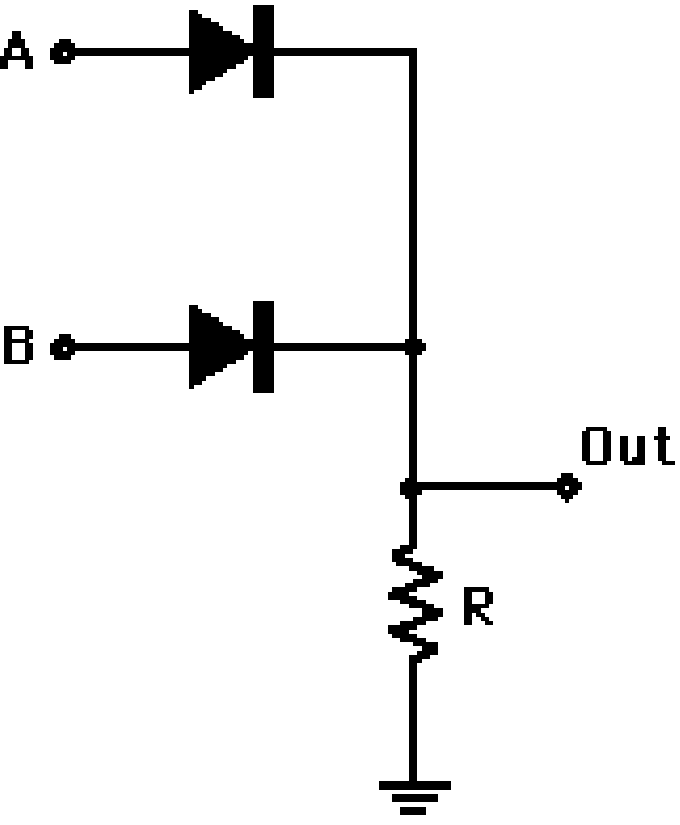
\includegraphics[width=0.17\linewidth]{img/OR_GATE.png}
    \caption{Diode OR gate}
    
\end{figure}

Vediamo i tre casi:

\begin{itemize}
    \item $V_A = V_B = 5V$
    \begin{itemize}
        \item entrambi i diodi conducono
        \item l'uscita va a 5V - $V_{on}$ (5 per grandi tensioni)
    \end{itemize}
    \item $V_A = 5V,  V_B = 0V$
    \begin{itemize}
        \item Il diodo A conduce, il diodo B è interdetto
        \item l'uscita va a 5V - $V_{on}$ (5 per grandi tensioni)
    \end{itemize}
    \item $V_A = V_B = 0V$
    \begin{itemize}
        \item entrambi i diodi sono interdetti
        \item l'uscita scende a 0V (0 per grandi tensioni)
    \end{itemize}
\end{itemize}


